\documentclass[12pt,a4paper]{article}

% Pacotes essenciais
\usepackage[utf8]{inputenc}
\usepackage[T1]{fontenc}
\usepackage[portuguese]{babel}
\usepackage{graphicx}
\usepackage{amsmath}
\usepackage{amssymb}
\usepackage{hyperref}
\usepackage{url}
\usepackage{indentfirst}
\usepackage{geometry}
\usepackage{setspace}
\usepackage{float}

% Configurações de página
\geometry{
    a4paper,
    left=3cm,
    right=2cm,
    top=3cm,
    bottom=2cm
}

% Configuração de espaçamento
\onehalfspacing

% Informações do documento
\title{\textbf{Google TPU (Tensor Processing Unit):\\Uma Análise da Arquitetura de Hardware Especializado\\para Aprendizado de Máquina}}
\author{
    Leonardo Heidi Almeida Murakami \\
    \small Universidade de São Paulo\\
    \small Instituto de Matemática e Estatística\\
    \small MAC0344 -- Arquitetura de Computadores\\
    \small Prof. Siang Wun Song
}
\date{Dezembro de 2024}

\begin{document}

\maketitle

\begin{abstract}
Este trabalho apresenta uma análise detalhada da Google Tensor Processing Unit (TPU), um circuito integrado de aplicação específica (ASIC) desenvolvido para acelerar operações de redes neurais e aprendizado de máquina. A TPU representa uma mudança de paradigma no processamento de cargas de trabalho de inteligência artificial, utilizando uma arquitetura sistólica (systolic array) que minimiza o acesso à memória e maximiza a eficiência energética. Através da análise de múltiplas gerações da TPU, desde sua introdução em 2015 até as versões mais recentes, este trabalho explora os princípios de design, características arquiteturais e vantagens de desempenho em comparação com processadores convencionais como CPUs e GPUs. Os resultados demonstram que a especialização de hardware pode proporcionar ganhos significativos de desempenho e eficiência energética para aplicações específicas, estabelecendo um novo caminho para o desenvolvimento de aceleradores de IA.

\textbf{Palavras-chave:} TPU, Tensor Processing Unit, ASIC, Systolic Array, Aprendizado de Máquina, Redes Neurais, Arquitetura de Computadores, Google.
\end{abstract}

\newpage
\tableofcontents
\newpage

\section{Introdução}

O avanço dos sistemas de inteligência artificial tem imposto demandas computacionais crescentes, especialmente para o treinamento e inferência de redes neurais profundas. Em 2013, projeções internas do Google indicaram que, caso cada usuário do Android utilizasse busca por voz por apenas três minutos diários, seria necessário dobrar a capacidade global de seus centros de dados \cite{google_tpu_blog_2017, thechipletter_2024}. Este cenário evidenciou limitações fundamentais das arquiteturas de processamento convencionais quando aplicadas em escala a cargas de trabalho de aprendizado de máquina.

As CPUs, projetadas como processadores de propósito geral, sofrem com o gargalo de von Neumann, que limita o desempenho em operações matriciais massivas devido à constante movimentação de dados entre memória e unidades de processamento \cite{google_cloud_tpu_docs}. As GPUs, embora ofereçam paralelismo massivo através de milhares de unidades aritméticas, mantêm características de propósito geral, incluindo hardware dedicado a cache, predição de desvios e renderização, que representam sobrecarga desnecessária para cargas de aprendizado de máquina \cite{datacamp_tpu_gpu_2024}.

Neste contexto, o Google desenvolveu a Tensor Processing Unit (TPU), um circuito integrado de aplicação específica (ASIC) projetado exclusivamente para acelerar operações de redes neurais. A TPU foi anunciada publicamente em maio de 2016, mas já operava internamente desde 2015 em serviços como Google Maps e Google Translate \cite{wikipedia_tpu_2024}. No núcleo de sua arquitetura encontra-se um \textit{systolic array}, uma matriz de unidades de multiplicação e acumulação (MACs) que executam operações matriciais de forma extremamente eficiente, baseada no conceito proposto por Kung e Leiserson em 1978 \cite{kung_leiserson_1978}. Os resultados iniciais foram expressivos: ganhos de 15 a 30 vezes em desempenho e de 30 a 80 vezes em eficiência energética comparados a CPUs e GPUs contemporâneas \cite{jouppi_tpu_paper_2017}.

Desde então, as TPUs evoluíram através de múltiplas gerações, expandindo sua aplicabilidade da inferência para o treinamento de modelos, e atualmente são disponibilizadas ao público através do serviço Cloud TPU \cite{google_cloud_tpu}. A geração mais recente, TPU v7, atinge 4,6 PetaFLOPS no formato BF16 \cite{techplanet_tpu_2024}.

O objetivo deste trabalho é apresentar uma análise da arquitetura e funcionamento das TPUs, explorando seus princípios de design, características técnicas e evolução ao longo das gerações. O trabalho está organizado da seguinte forma: a Seção 2 apresenta os fundamentos teóricos das operações em redes neurais; a Seção 3 detalha a arquitetura da TPU e o \textit{systolic array}; e a Seção 4 apresenta as considerações finais, incluindo a evolução das gerações e perspectivas futuras.

\section{Fundamentos Teóricos}

As redes neurais artificiais realizam tarefas de aprendizado através de operações matemáticas aplicadas sobre seus parâmetros internos. Compreender essas operações é fundamental para entender por que arquiteturas especializadas como a TPU podem oferecer vantagens significativas de desempenho. Esta seção apresenta as operações matemáticas fundamentais em redes neurais e como elas se relacionam com multiplicação de matrizes.

\subsection{Operações Fundamentais em Redes Neurais}

Uma rede neural consiste em camadas de neurônios artificiais organizados sequencialmente. Cada neurônio recebe entradas, aplica uma transformação linear seguida de uma função de ativação não-linear, e propaga o resultado para a próxima camada. Matematicamente, a operação em um neurônio individual pode ser descrita como:

\begin{equation}
a = \sigma(w^T x + b)
\end{equation}

onde $x$ é o vetor de entrada, $w$ é o vetor de pesos, $b$ é o termo de viés (bias), $\sigma$ é a função de ativação, e $a$ é a saída (ativação) do neurônio.

Para uma camada completa com múltiplos neurônios, essa operação se generaliza para a forma matricial:

\begin{equation}
A^{[l]} = \sigma(W^{[l]} A^{[l-1]} + b^{[l]})
\end{equation}

onde $A^{[l]} \in \mathbb{R}^{n_l \times m}$ representa as ativações da camada $l$, $W^{[l]} \in \mathbb{R}^{n_l \times n_{l-1}}$ é a matriz de pesos, $b^{[l]} \in \mathbb{R}^{n_l \times 1}$ é o vetor de viés, $n_l$ é o número de neurônios na camada $l$, e $m$ é o número de exemplos no mini-batch. A função de ativação $\sigma$ é aplicada elemento a elemento.

\subsection{Propagação Direta (Forward Propagation)}

A propagação direta é o processo pelo qual os dados de entrada atravessam a rede neural para produzir uma saída. Para uma rede neural com $L$ camadas, este processo pode ser expresso como uma sequência de multiplicações matriciais:

\begin{align}
Z^{[1]} &= W^{[1]} X + b^{[1]} \\
A^{[1]} &= \sigma^{[1]}(Z^{[1]}) \\
Z^{[2]} &= W^{[2]} A^{[1]} + b^{[2]} \\
A^{[2]} &= \sigma^{[2]}(Z^{[2]}) \\
&\vdots \\
Z^{[L]} &= W^{[L]} A^{[L-1]} + b^{[L]} \\
\hat{Y} &= A^{[L]} = \sigma^{[L]}(Z^{[L]})
\end{align}

onde $X \in \mathbb{R}^{n_0 \times m}$ é a matriz de entrada contendo $m$ exemplos, cada um com $n_0$ características. O termo $Z^{[l]}$ representa a combinação linear antes da ativação, enquanto $A^{[l]}$ representa as ativações após aplicar a função não-linear.

A característica fundamental deste processo é que ele consiste essencialmente de operações de multiplicação matriz-matriz (GEMM - General Matrix Multiplication), intercaladas com aplicações de funções não-lineares. Em redes profundas modernas, essas multiplicações matriciais representam mais de 90\% do custo computacional total \cite{jouppi_tpu_paper_2017}.

\subsection{Retropropagação (Backpropagation)}

O treinamento de redes neurais utiliza o algoritmo de retropropagação para calcular os gradientes da função de custo em relação aos parâmetros da rede. Este algoritmo também se baseia fundamentalmente em multiplicações matriciais. Dado um custo $J$, os gradientes são calculados através da regra da cadeia:

\begin{align}
\frac{\partial J}{\partial W^{[l]}} &= \frac{\partial J}{\partial Z^{[l]}} \frac{\partial Z^{[l]}}{\partial W^{[l]}} = \delta^{[l]} (A^{[l-1]})^T \\
\frac{\partial J}{\partial b^{[l]}} &= \delta^{[l]} \\
\delta^{[l-1]} &= (W^{[l]})^T \delta^{[l]} \odot \sigma'^{[l-1]}(Z^{[l-1]})
\end{align}

onde $\delta^{[l]} = \frac{\partial J}{\partial Z^{[l]}}$ é o erro da camada $l$, e $\odot$ denota o produto de Hadamard (multiplicação elemento a elemento). Novamente, as operações dominantes são multiplicações matriciais: $\delta^{[l]} (A^{[l-1]})^T$ para o gradiente dos pesos e $(W^{[l]})^T \delta^{[l]}$ para propagar o erro.

\subsection{Camadas Convolucionais}

Redes neurais convolucionais (CNNs) utilizam camadas convolucionais que aplicam filtros sobre janelas locais da entrada. Uma operação de convolução 2D pode ser expressa como:

\begin{equation}
Y_{i,j,k} = \sum_{c=1}^{C} \sum_{p=0}^{F-1} \sum_{q=0}^{F-1} X_{i+p, j+q, c} \cdot K_{p,q,c,k} + b_k
\end{equation}

onde $X$ é a entrada de dimensões $(H \times W \times C)$, $K$ é o filtro de dimensões $(F \times F \times C \times M)$, $C$ é o número de canais de entrada, $M$ é o número de filtros, $F$ é o tamanho do filtro, e $Y$ é a saída de dimensões $(H' \times W' \times M)$.

Embora conceitualmente diferente de uma multiplicação matricial direta, a convolução pode ser reformulada como multiplicação de matrizes através da transformação \textit{im2col} (image-to-column). Esta técnica desdobra patches da imagem em colunas de uma matriz, permitindo que a convolução seja expressa como:

\begin{equation}
Y_{col} = K_{reshaped} \cdot X_{col}
\end{equation}

onde $X_{col} \in \mathbb{R}^{(F \times F \times C) \times (H' \times W')}$ é a matriz resultante de desdobrar os patches da imagem, e $K_{reshaped} \in \mathbb{R}^{M \times (F \times F \times C)}$ é a matriz de filtros reorganizada. Esta transformação é amplamente utilizada em frameworks de deep learning como Caffe, PyTorch e TensorFlow, pois permite aproveitar implementações otimizadas de multiplicação matricial \cite{chellapilla_gemm_2006}.

A desvantagem do \textit{im2col} é que ele replica dados de entrada, aumentando o uso de memória por um fator de aproximadamente $F^2$ para filtros de tamanho $F \times F$. No entanto, a eficiência computacional das multiplicações matriciais resultantes geralmente compensa este custo adicional de memória.

\subsection{Dominância das Operações Matriciais}

A análise de cargas de trabalho em redes neurais modernas revela que as multiplicações matriciais dominam o tempo de execução. Por exemplo, em arquiteturas como ResNet-50, VGG-16, e modelos de linguagem baseados em Transformers, a grande maioria das operações de ponto flutuante (FLOPs) são atribuídas a multiplicações matriz-matriz e matriz-vetor \cite{jouppi_tpu_paper_2017}.

Esta dominância de operações matriciais tem implicações importantes para o design de hardware:

\begin{itemize}
\item \textbf{Reutilização de dados}: Em uma multiplicação matriz-matriz $C = AB$, cada elemento de $A$ e $B$ é usado múltiplas vezes. Um elemento $A_{i,k}$ é multiplicado por todos os elementos da linha $k$ de $B$, e similarmente para $B_{k,j}$.

\item \textbf{Paralelismo}: As operações de multiplicação e acumulação (MACs) podem ser executadas de forma massivamente paralela, já que muitas delas são independentes entre si.

\item \textbf{Padrões de acesso à memória}: O padrão de acesso aos dados em multiplicações matriciais é regular e previsível, permitindo otimizações específicas de hardware.
\end{itemize}

Essas características tornam a multiplicação matricial uma operação ideal para especialização de hardware. Ao projetar um acelerador que executa multiplicações matriciais de forma extremamente eficiente, é possível acelerar significativamente toda a computação de redes neurais. Este é precisamente o princípio fundamental por trás da arquitetura da TPU, que dedica a maior parte de seus recursos de silício para um único propósito: executar multiplicações matriciais da forma mais eficiente possível em termos de desempenho e energia.

\section{Arquitetura da TPU}

Esta seção apresenta a arquitetura da primeira geração da TPU (TPU v1), destacando seus componentes principais e o funcionamento do \textit{systolic array}. A TPU v1 foi projetada especificamente para inferência de redes neurais, priorizando eficiência energética e throughput sobre flexibilidade.

\subsection{Visão Geral da TPU v1}

A TPU v1 é um ASIC fabricado em processo de 28 nm com área de die inferior a 331 mm² \cite{wikipedia_tpu_2024}. Opera a 700 MHz com consumo térmico de 28--40 W, conectando-se ao processador host via interface PCIe 3.0. A escolha de uma frequência relativamente baixa foi deliberada, priorizando eficiência energética sobre desempenho bruto por chip.

O chip utiliza uma arquitetura CISC (Complex Instruction Set Computer) com aproximadamente 20 instruções, enviadas pelo processador host através do barramento PCIe. As cinco instruções principais são: \texttt{Read\_Host\_Memory} (lê dados da memória do host para o Unified Buffer), \texttt{Read\_Weights} (carrega pesos da memória de pesos para o Weight FIFO), \texttt{MatrixMultiply/Convolve} (executa multiplicação matricial ou convolução), \texttt{Activate} (aplica funções de ativação), e \texttt{Write\_Host\_Memory} (escreve resultados de volta ao host) \cite{jouppi_tpu_paper_2017}.

\subsection{Componentes Principais}

A arquitetura da TPU v1 pode ser dividida nos seguintes componentes principais, ilustrados na Figura \ref{fig:tpu_architecture}:

\begin{figure}[H]
    \centering
    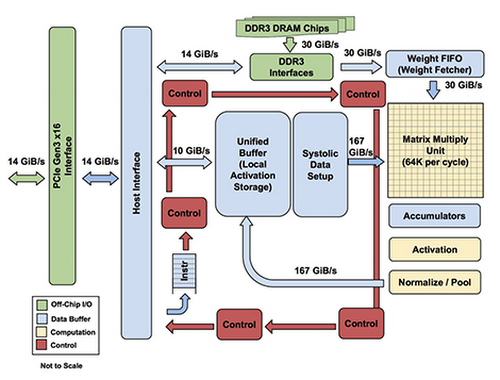
\includegraphics[width=0.65\textwidth]{images/tpu-architecture.png}
    \caption{Diagrama simplificado da arquitetura da TPU v1, destacando a conexão entre memória de pesos, Unified Buffer, Matrix Multiply Unit (systolic array), acumuladores e a unidade de ativação. Adaptado de \cite{google_tpu_blog_2017}.}
    \label{fig:tpu_architecture}
\end{figure}

\textbf{Memória de Pesos:} 8 GiB de DRAM DDR3-2133 dual-channel off-chip, oferecendo 34 GB/s de largura de banda. Os pesos são pré-carregados nesta memória a partir do host via PCIe, permanecendo disponíveis para múltiplas operações de inferência. Um Weight FIFO on-chip de quatro camadas faz interface entre a memória externa e a unidade de multiplicação matricial.

\textbf{Unified Buffer:} Memória on-chip de 24 MiB que armazena as ativações intermediárias. Esta memória serve como buffer principal para dados de entrada e saídas intermediárias das camadas da rede neural, ocupando aproximadamente 30\% da área do chip. Conecta-se diretamente à Matrix Multiply Unit através de um barramento de 256 bytes de largura com 167 GiB/s de largura de banda.

\textbf{Matrix Multiply Unit (MXU):} O componente central da TPU, consistindo em um \textit{systolic array} de 256×256 unidades de multiplicação e acumulação (MACs), totalizando 65.536 MACs operando em paralelo. Cada MAC executa multiplicações de inteiros de 8 bits, produzindo produtos de 16 bits que são acumulados em registradores de 32 bits. A 700 MHz, o MXU pode executar $65.536 \times 700.000.000 = 46 \times 10^{12}$ operações de multiplicação-acumulação por segundo, equivalente a 92 TOPS (tera operações por segundo) \cite{google_tpu_blog_2017}.

\textbf{Acumuladores:} 4 MiB de memória organizada em 4.096 vetores de 256 elementos de 32 bits cada. Coletam os produtos de 16 bits da MXU e realizam acumulação em precisão de 32 bits, prevenindo overflow durante somas longas. O dimensionamento para 4.096 vetores (com arredondamento para 2.048 duplicado para double buffering) foi baseado em observações empíricas de que o desempenho máximo era atingido em torno de 1.350 vetores.

\textbf{Activation Unit:} Pipeline de ativação que aplica funções não-lineares comuns em redes neurais, como ReLU, sigmoid e tanh, além de operações de normalização e pooling. Este componente oferece suporte em hardware para estas operações, que embora menos intensivas computacionalmente que multiplicações matriciais, ocorrem com alta frequência.

\subsection{Arquitetura Sistólica (Systolic Array)}

O conceito de \textit{systolic array}, proposto originalmente por Kung e Leiserson em 1978, é fundamental para a eficiência da TPU. O termo "sistólico" refere-se ao fluxo rítmico de dados através do chip, análogo ao bombeamento de sangue pelo coração.

Na TPU v1, o \textit{systolic array} é implementado como uma grade 256×256 de MACs interconectados. O funcionamento segue um padrão weight-stationary (pesos estacionários):

\begin{enumerate}
\item Os pesos da matriz $W \in \mathbb{R}^{256 \times 256}$ são pré-carregados e fixados nas unidades MAC do array.

\item As ativações de entrada $A \in \mathbb{R}^{B \times 256}$ (onde $B$ é o tamanho do batch) fluem horizontalmente da esquerda para a direita através do array.

\item Cada MAC multiplica sua ativação de entrada pelo peso armazenado e adiciona o resultado a uma soma parcial que chega verticalmente de cima.

\item As somas parciais fluem verticalmente de cima para baixo através do array.

\item Os resultados finais emergem na parte inferior do array após $B$ ciclos de pipeline.
\end{enumerate}

A vantagem crítica desta arquitetura é a eliminação de acessos intermediários à memória. Durante toda a multiplicação matricial, os dados fluem diretamente entre MACs adjacentes sem armazenamento temporário. Cada peso é lido da memória uma única vez e reutilizado para múltiplas ativações, e cada ativação atravessa o array sendo multiplicada por todos os pesos relevantes. Esta reutilização massiva de dados, combinada com o acesso mínimo à memória, resulta na excepcional eficiência energética da TPU.

Para uma operação de multiplicação matricial $C = A \times W$, onde $A$ é $B \times 256$ e $W$ é $256 \times 256$, o \textit{systolic array} completa a operação em $B$ ciclos (após um período inicial de preenchimento do pipeline). Compare isso com uma CPU que precisaria realizar $B \times 256 \times 256$ acessos à memória e o mesmo número de operações sequenciais.

\subsection{Pipeline e Execução de Instruções}

A TPU implementa um pipeline de 4 estágios para instruções CISC, permitindo sobreposição da execução de diferentes instruções. O objetivo é manter a MXU constantemente ocupada, escondendo a latência das outras operações. A instrução \texttt{MatrixMultiply} é particularmente importante: possui 12 bytes, dos quais 3 bytes são endereço do Unified Buffer, 2 bytes são endereço do acumulador, 4 bytes são comprimento (às vezes 2 dimensões para convoluções), e o restante é opcode e flags.

A filosofia decoupled-access/execute é seguida pela instrução \texttt{Read\_Weights}, que envia o endereço antes da busca dos pesos da memória. Durante operações típicas, as instruções de leitura de pesos e leitura de dados do host são sobrepostas com a execução da multiplicação matricial na MXU, maximizando a utilização do hardware.

\subsection{Desempenho e Eficiência}

A TPU v1 demonstrou ganhos significativos sobre processadores convencionais. Comparada com CPUs Intel Haswell e GPUs NVIDIA K80 contemporâneas, a TPU v1 apresentou desempenho 15 a 30 vezes superior em cargas de inferência de redes neurais e eficiência energética 30 a 80 vezes maior, alcançando aproximadamente 2,3 TOPS/W \cite{jouppi_tpu_paper_2017}.

Estas melhorias derivam diretamente das escolhas arquiteturais: especialização para multiplicação matricial, eliminação de hardware desnecessário para propósito geral, minimização de acessos à memória através do \textit{systolic array}, e operação em precisão reduzida (8 bits) adequada para inferência.

A TPU v1 foi empregada em diversos serviços do Google, incluindo processamento de texto no Google Street View (analisando toda a base de dados em menos de cinco dias), Google Photos (processando mais de 100 milhões de fotos por dia por chip), RankBrain (para resultados de busca), e no sistema AlphaGo, que derrotou o campeão mundial de Go, Lee Sedol, em 2016 \cite{wikipedia_tpu_2024}.

\section{Considerações Finais}

Este trabalho apresentou a Google Tensor Processing Unit (TPU), demonstrando como a especialização de hardware pode proporcionar ganhos substanciais em desempenho e eficiência energética para cargas de trabalho específicas. A análise da arquitetura da TPU v1 revelou que seus ganhos derivam de decisões arquiteturais fundamentais: dedicação de recursos quase exclusivos para multiplicação matricial, uso de \textit{systolic array} para minimizar acessos à memória, e operação em precisão reduzida adequada para inferência.

\subsection{Evolução e Impacto}

As TPUs evoluíram significativamente desde 2015. A v2 (2017) introduziu ponto flutuante e o formato bfloat16, expandindo do foco original em inferência para incluir treinamento. Com 16 GB de HBM e 45 teraFLOPS por chip, pods de 256 chips atingiam 11,5 petaFLOPS \cite{wikipedia_tpu_v2}. A v3 dobrou o desempenho por chip e quadruplicou chips por pod (1.024 chips). A v4 (2021) trouxe interconexão ICI com 10 vezes a largura de banda anterior, suportando pods de 4.096 chips. As versões recentes v5e, v5p, v6e (com \textit{systolic array} 256×256) e v7 continuam avançando, com a v7 atingindo 4.614 TFLOPS em BF16 \cite{techplanet_tpu_2024}.

O impacto prático é substancial: TPUs processam bilhões de requisições diárias em Google Translate, ranqueamento de busca, Google Photos e YouTube. A empresa de veículos autônomos Waymo utiliza TPUs para treinar redes neurais antes de testar seus modelos através de simulações, permitindo que os modelos processem grandes volumes de dados e reajam ao ambiente do veículo em tempo real \cite{builtin_tpu_2024}. Mais importante, TPUs viabilizaram economicamente serviços de IA em escala que seriam proibitivos com hardware convencional.

\subsection{Tendências e Perspectivas}

A TPU catalisou uma tendência ampla na indústria. NVIDIA desenvolveu Tensor Cores; Intel desenvolve Habana Gaudi; startups como Groq (fundada por engenheiros originais da TPU), Cerebras e Graphcore propõem arquiteturas alternativas. Duas tendências merecem destaque: SparseCores para acelerar embeddings em modelos de recomendação, e Edge TPU para computação de borda com restrições severas de energia.

Modelos de linguagem de grande escala apresentam características diferentes de CNNs tradicionais, com ênfase em operações de atenção. Aceleradores futuros provavelmente incorporarão unidades especializadas para estes padrões. Técnicas como quantização extrema (4 bits ou menos) podem permitir ganhos adicionais de eficiência.

\subsection{Lições Fundamentais}

A TPU oferece três lições importantes. Primeira, uma especialização extrema produz ganhos de ordem de magnitude quando aplicada a domínios bem definidos. Segunda, inovações arquiteturais fundamentais superam ganhos incrementais em frequência ou processo de fabricação. Terceira, o co-design entre algoritmos e hardware é essencial: a eficácia da TPU deriva de que redes neurais executam predominantemente multiplicações matriciais.

A TPU demonstra que o fim da lei de Moore não significa o fim do progresso em computação. Aceleradores especializados abrem novos caminhos para ganhos de desempenho e eficiência, paradigma que provavelmente se estenderá para processamento de grafos, criptografia, simulação científica e outros domínios.

Em conclusão, a TPU representa um marco na arquitetura de computadores, validando a especialização como estratégia viável para superar limitações de processadores de propósito geral. À medida que a inteligência artificial permeia mais aspectos da computação moderna, aceleradores especializados tornam-se essenciais para viabilizar aplicações impraticáveis com hardware convencional.

\newpage

\begin{thebibliography}{99}

\bibitem{google_tpu_blog_2017}
SATO, Kaz; YOUNG, Cliff.
\textit{An in-depth look at Google's first Tensor Processing Unit (TPU)}.
Google Cloud Blog, maio 2017.
Disponível em: \url{https://cloud.google.com/blog/products/ai-machine-learning/an-in-depth-look-at-googles-first-tensor-processing-unit-tpu}.
Acesso em: dezembro 2025.

\bibitem{thechipletter_2024}
\textit{Google's First Tensor Processing Unit: Origins}.
The Chip Letter, fevereiro 2024.
Disponível em: \url{https://thechipletter.substack.com/p/googles-first-tensor-processing-unit}.
Acesso em: dezembro 2025.

\bibitem{google_cloud_tpu_docs}
GOOGLE CLOUD.
\textit{Introduction to Cloud TPU}.
Google Cloud Documentation, 2024.
Disponível em: \url{https://cloud.google.com/tpu/docs/intro-to-tpu}.
Acesso em: dezembro 2025.

\bibitem{datacamp_tpu_gpu_2024}
PYKES, Kurtis. 
\textit{Understanding TPUs vs GPUs in AI: A Comprehensive Guide}.
DataCamp, maio 2024.
Disponível em: \url{https://www.datacamp.com/blog/tpu-vs-gpu-ai}.
Acesso em: dezembro 2025.

\bibitem{wikipedia_tpu_2024}
\textit{Tensor Processing Unit}.
Wikipedia, dezembro 2025.
Disponível em: \url{https://en.wikipedia.org/wiki/Tensor_Processing_Unit}.
Acesso em: dezembro 2025.

\bibitem{thechipletter_retrospective}
\textit{Google's First Tensor Processing Unit - Architecture}.
The Chip Letter, março 2024.
Disponível em: \url{https://thechipletter.substack.com/p/googles-first-tpu-architecture}.
Acesso em: dezembro 2025.

\bibitem{kung_leiserson_1978}
KUNG, H. T.; LEISERSON, Charles E.
\textit{Systolic Arrays (for VLSI)}.
Sparse Matrix Proceedings 1978, Carnegie Mellon University, 1978.

\bibitem{jouppi_tpu_paper_2017}
JOUPPI, Norman P. et al.
\textit{In-Datacenter Performance Analysis of a Tensor Processing Unit}.
Proceedings of the 44th Annual International Symposium on Computer Architecture (ISCA), 2017.

\bibitem{wikipedia_tpu_v2}
\textit{Tensor Processing Unit --- Second Generation}.
Wikipedia, dezembro 2025.
Disponível em: \url{https://en.wikipedia.org/wiki/Tensor_Processing_Unit#Second_generation}.
Acesso em: dezembro 2025.

\bibitem{techplanet_tpu_2024}
KELLY.
\textit{Google's Secret Weapon: How TPUs Could Win the Long-Term AI Race Against NVIDIA}.
TechPlanet, dezembro 2024.
Disponível em: \url{https://techplanet.today/post/googles-secret-weapon-how-tpus-could-win-the-long-term-ai-race-against-nvidia}.
Acesso em: dezembro 2025.

\bibitem{google_cloud_tpu}
GOOGLE CLOUD.
\textit{Tensor Processing Units (TPUs)}.
Google Cloud, 2024.
Disponível em: \url{https://cloud.google.com/tpu}.
Acesso em: dezembro 2025.

\bibitem{chellapilla_gemm_2006}
CHELLAPILLA, Kumar; PURI, Sidd; SIMARD, Patrice.
\textit{High Performance Convolutional Neural Networks for Document Processing}.
Tenth International Workshop on Frontiers in Handwriting Recognition, 2006.

\bibitem{builtin_tpu_2024}
URWIN, Matthew.
\textit{What Is a Tensor Processing Unit (TPU)?}
Built In, 2024.
Disponível em: \url{https://builtin.com/articles/tensor-processing-unit-tpu}.
Acesso em: dezembro 2025.

\end{thebibliography}

\end{document}